\documentclass{report}

\usepackage{amsmath}
\usepackage{amsfonts}
\usepackage{amsthm}

\theoremstyle{plain}
\newtheorem{thm}{Theorem}[section]
\newtheorem{lem}[thm]{Lemma}
\newtheorem{prop}[thm]{Proposition}
\newtheorem*{cor}{Corollary}

\theoremstyle{definition}
\newtheorem{defn}{Definition}[section]
\newtheorem{conj}{Conjecture}[section]
\newtheorem{exmp}{Example}[section]

\theoremstyle{remark}
\newtheorem*{rem}{Remark}
\newtheorem*{note}{Note}

\usepackage{systeme}

\usepackage{tikz}
\usetikzlibrary{arrows,decorations.markings}
\usetikzlibrary{cd}


\usepackage{etoolbox}
\listadd{\pc}{$C$}
\listadd{\pc}{$C\sharp$}
\listadd{\pc}{$D$}
\listadd{\pc}{$E\flat$}
\listadd{\pc}{$E$}
\listadd{\pc}{$F$}
\listadd{\pc}{$F\sharp$}
\listadd{\pc}{$G$}
\listadd{\pc}{$G\sharp$}
\listadd{\pc}{$A$}
\listadd{\pc}{$B\flat$}
\listadd{\pc}{$B$}
\usepackage{calc}

\usepackage[top=2.5cm, left=3cm, right=3cm, bottom=2.5cm]{geometry}
\usepackage{caption}
\usepackage{hyperref}
\captionsetup{margin=10pt,font=small,labelfont=bf}

\usepackage{floatrow}
\newenvironment{tzfigure}[1]
{
    \begin{figure}[h]
        \centering
        #1
        \begin{tikzpicture}
}
{
        \end{tikzpicture}   
    \end{figure}
}

\newenvironment{tzcategory}[1]
{
    \begin{figure}[h]
        \centering
        #1
        \begin{tikzpicture}[baseline= (a).base]    
}
{
    \end{tikzpicture}   
\end{figure}
}


\begin{document}

%\begingroup    

\title{Categories and music}
\author{Alice Rixte}
\date{\today}
\maketitle %\endgroup


\chapter{Introduction}


\section{Presentation of Allen Forte's work}
\begin{defn}
    A \textbf{pitch class} consists of all the pitches separated with a whole number of octaves.
\end{defn}
The set of all pitch classes comes naturally with a group structure, which is actually the group $\mathbb{Z}_{12}$. Indeed, we can associate $C$ to the pitch class $0$, $C\sharp$ to the pitch class $1$ and so on. We then have the possibillity to represent a $C$ major chord  from a geometrical point of vue (see \hyperref[Cmajor]{Figure \ref*{Cmajor}}).

\newcounter{itemcount}
\setcounter{itemcount}{450}
\renewcommand*{\do}[1]{
    \filldraw [black]  (\number\value{itemcount}:3cm) circle (1.5pt)
    node[anchor={\number\value{itemcount}-180}]
        {#1\addtocounter{itemcount}{-30}};
}
\begin{tzfigure}{
        \caption{The C Major chord in the chromatic circle}
        \label{Cmajor}
    }
    \dolistloop{\pc}
    \draw[fill=blue!20] (90:3cm) -- (330:3cm) -- (240:3cm) -- cycle;
    \draw [domain=0:360,samples=60] plot ({3*cos(\x)}, {3*sin(\x)});
\end{tzfigure}

The idea of Forte relies on the fact that a major chord will always have the same representation up to 12 rotations in this geometrical paradigm. In mathematics they are the 12 rotational symmetries of the regular dodecahedron.In music theory, these rotations are called \textbf{transpositions} and are named $T_i$ for $i\in[\![0,11]\!]$.

His intuition was that instead of considering triads (three notes chord) as the set of the notes that compose them, we should consider them as the set of the intervals between each note. As a result, every inversion of chord \footnote{the term inversion has to be taken here from a musical point of view, for instance the inversions of a C major chord are C-E-G, G-C-E, E-G-C. Later in this report, we will use inversion with another definition and we will stick to it.} will be in the same \textbf{pitch-class set}\cite{forte_1980}. This can be seen in the geometrical point of view where the simple fact  of representing the chord as a triangle allow to forget any order between the three note. Similarly, all the transpositions of the chord will be in the same pitch-class.

\paragraph{Contribution (sort of)}
From another point of view, the work of Forte can be seen as networks, as in \hyperref[transpose_net]{Figure \ref*{transpose_net}}. Nonetheless, this representation does not allow for the moment to embed the notion of pitch-class set of Forte. For this we have to introduce the Klumpenhouwer networks.
\begin{tzcategory}{
        \caption{Transpositional network}
        \label{transpose_net}
    }
    \node[scale=1.3] (a) at (0,0){
        \begin{tikzcd}
            G                                                            \\
            E \arrow[u, "T_3", bend left]                                \\
            C \arrow[u, "T_4", bend left] \arrow[uu, "T_7"', bend right]
        \end{tikzcd}};
\end{tzcategory}



\section{Presentation of Klumpenhouwer networks}
In  the 1980s, David Lewin developped a branch of music theory called transformational theory\cite{rahn_lewin_1987}. It consists of, rather than looking the musical objects for themselves but instead to mathematically study the relation between them.
%TODO read rahn_lewin_1987

Klumpenhouwer networks, or K-nets, were then introduced by Henry Klumpenhouwer, former PhD student of Lewin, to formalize the relation between two chords\cite{lewin_1990}.

We have seen that the rotations of the dodecahedron match with the notion of transposition. However, there another type of symmetry in the dodecahedron : the $12$ reflexion symmetries (see\hyperref[inversions]{Figure \ref*{inversions}}), called \textbf{inversions} in transformational music theory. Along with transposition, they form the $T/I$ group, otherwise known in mathematics as the \textbf{dihedral group} of a dodecahedron.

\setcounter{itemcount}{450}

\begin{tzfigure}{
        \caption{The $I_0$ inversion}
        \label{inversions}
    }
    \tikzset{myptr/.style={decoration={markings,mark=at position 1 with
                            {\arrow[scale=3,>=stealth]{>}}},postaction={decorate}}}
    \dolistloop{\pc}
    \draw [domain=0:360,samples=60] plot ({3*cos(\x)}, {3*sin(\x)});
    \draw [dashed,purple] (90:3cm) -- (270:3cm);
    \foreach \i in {1,...,5}{
            \draw [<->, >=stealth, thick, purple] (90 + \i*30:3cm) -- (90-\i*30:3cm) ;
        }
\end{tzfigure}


The idea behind K-nets is that instead of analyse chords transformations threw transposition only, which is not very rich, we could instead use also inversions.

\begin{defn}
    A Klumpenhouwer network is a network where objects are pitch classes and arrows between objects are labeled by an element of the group $T/I$.
\end{defn}

\begin{defn}
    Two K-nets $K$ and $K'$ are said \textbf{isographic} if and only if :
    \begin{itemize}
        \item there exist a bijection $f:V(K)\rightarrow V(K')$ from the set of vertices $V(K)$ to $V(K')$
        \item if there is an arrow $a:s\rightarrow t$ where $s,t\in V(K)$ in $K$, then there is an arrow $a':f(s)\rightarrow f(t)$ in $K'$
        \item there is an automorphism $F \in Aut(T/I)$ such that if $X$ is the label of an arrow $a:s\rightarrow t$, then $F(X)$ is the label of the arrow $a':f(s)\rightarrow f(t)$.
    \end{itemize}
\end{defn}




\section{Presentation of PK-nets}

PK-nets\cite{PAAE2016} are a generalization of K-nets. They are defined in the paradigm of category theory. Let's first present informally category theory.

The concept of category theory is simply summarized by the french proverb "Tell me who your friends are and I'll tell you who you are." The idea is that, in mathematics, it can be more important to consider the relations between objects than look at the objects themselves.

Another concept fundamental of category theory is composition.
%TODO


\begin{defn}\textbf{Set} is the category where objects are the sets and morphisms are functions between sets.
    \begin{figure}
        \centering
        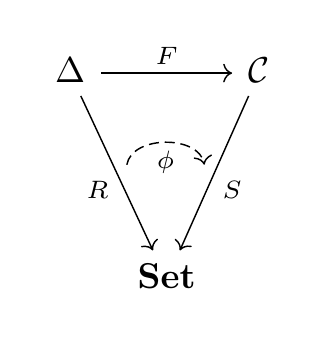
\begin{tikzpicture}[baseline= (a).base]
            \node[scale=1.3] (a) at (0,0){
                \begin{tikzcd}[column sep=tiny]
                    \Delta
                    \ar[ddr, "R"',""{name=R,right}]
                    \ar[rr,"F"]
                    & &
                    \mathcal{C}
                    \ar[ddl,"S",""{name=S,left}] \\
                    & \ar[dashed,bend left=80,from=R, to=S, "\phi"']& \\
                    & \bf Set &
                \end{tikzcd}
            };
        \end{tikzpicture}
        \caption{PK-net definition}
    \end{figure}
\end{defn}

\begin{tzcategory}{\caption{PK-net definition}}
    % \node[scale=1.3] (a) at (0,0){
    \begin{tikzcd}[column sep=tiny]
        \Delta
        \ar[ddr, "R"',""{name=R,right}]
        \ar[rr,"F"]
        & &
        \mathcal{C}
        \ar[ddl,"S",""{name=S,left}] \\
        & \ar[dashed,bend left=80,from=R, to=S, "\phi"']& \\
        & \bf Set &
    \end{tikzcd}
    % };
\end{tzcategory}





The definition of a PK-net is very general and covers a lot of the concepts introduced, such as (TODO) transposition class, Lewin's GIS (TODO), Forte's (TODO) normal order class, , (TODO) K-nets, symmetric groups of permutations (TODO), Tonnetz...

\paragraph{Contribution (sort of)}

Let's study a particular class of PK-nets such that $\Delta$, $\mathcal{C}$, $R$ and $S$ are fixed. The only thing we are allowed to change is $F$.

\begin{prop}
    Let $F' : \Delta \rightarrow \mathcal{C}$ such that there exist a natural transformation $\psi : F \rightarrow F'$, then we get an obvious natural transformation $\phi' : R \rightarrow SF$
\end{prop}
\begin{proof}
    Let $\phi'_A : R(A) \rightarrow SF'(A)$ such that, $\phi'_A = S\psi_A$. In other words, in the category of functors, $\phi' = Id_S\psi$ which is necessarily a natural transformation, due to the axioms of the category of functors.
    \begin{tzcategory}{}
        \node[scale=1.3] (a) at (0,0){
            \begin{tikzcd}[column sep = small, row sep = 5.5ex]
                \Delta
                \arrow[bend left=40]{rr}[name=F,label=above:$F$]{}
                \arrow[bend right=40]{rr}[name=F2,label=below:$F'$]{}
                \ar[ddr, "R"',""{name=R,right}]
                & &
                \mathcal{C}
                \arrow[shorten <=5pt,shorten >=0pt,Rightarrow,to path={(F) -- node[label=right:$\psi$] {} (F2)}]{}
                \ar[ddl,"S",""{name=S,left}] \\
                & & \\
                & \textbf{Set}&
            \end{tikzcd}
        };
    \end{tzcategory}
\end{proof}

\subsection{Study of $\psi$}

Let $F:\Delta\rightarrow G$ and $F':\Delta\rightarrow G$ be two parallel functors where $G\in \textbf{Grp}$. Let $X,Y\in\Delta$ and $f\in Hom(X,Y)$. We then get the following commutating diagram :

\begin{tzcategory}{}
    \node[scale=1.3] (a) at (0,0){
        \begin{tikzcd}[column sep = small]
            F(X) \arrow[dd, "F(f)"'] \arrow[rr, "\psi_X"] &  & F'(X) \arrow[dd, "F'(f)"] \\
            &  &                           \\
            F(Y) \arrow[rr, "\psi_Y"']                    &  & F'(Y)
        \end{tikzcd}
    };
\end{tzcategory}


This diagrams corresponds to the equation :
\begin{eqnarray*}
    &a\cdot y &= x \cdot b\\
    \Leftrightarrow & y &= a^{-1}\cdot x\cdot  b\\
\end{eqnarray*}

Hence, there is no constraint on the couple $(x,y)$, we juste need to choose $a = x$ and $b = y$, and we get our natural transformation.

Though, $X$ and $Y$ are actually the same object and $f$ is a reflexive object, we get $a = b$, and consequently,
$$y = b^{-1}\cdot x \cdot b $$

In other words, $\psi$ is an \textbf{inner automorphism} of $G$.


\chapter{EK-nets}
% \subsection{$\mathhcal{C}$ is a one-object category}
% A natural transformation of $\Delta$ to $M$ associates each object of $\Delta$ to an arrow of $M$, i.e.an element of the underlying monoid.

We are particularly interested in the case where $\mathcal{C} = T/I$. Since $T/I$ has only one element, all the functors $F:\Delta \rightarrow T/I$ send all the elements on the unique element of $T/I$. In the following, we will not recall the image of the elements of $\Delta$.

Moreover, we ask that

\begin{equation}
    \forall X, Y\in \Delta, \forall f, g \in Hom(X,Y), F(f) = F(g) \Rightarrow f = g
    \label{Fcondition}
\end{equation}
%TODO define group action
Here, $S:\mathcal{C}\rightarrow \textbf{Set}$ is the action of $T/I$ on the set $Notes = \{C,C\sharp,D,E\flat,E,F,F\sharp,G\sharp,A,B\flat,B\}$.

Let us study what shape the category $\Delta$ could have. It can of course be void, since the empty category is the initial object of $\textbf{Cat}$.

\section{Recover pitch classes}
%TODO : better proof
Let us suppose that $\Delta$ has only one element $A$. Then the \hyperref[Fcondition]{Condition \ref*{Fcondition}} implies that $F$ is a monomorphism in the $\textbf{Grp}$ category. Consequently, $\Delta$ is isomorphic to a subgroup of $T/I$. Each of these subgroups is in one-to-one correspondance with the functors $F$ following the \hyperref[Fcondition]{Condition \ref*{Fcondition}}.

\paragraph{$\Delta$ has exactly one arrow}
Let us suppose $\Delta$ has only one arrow : the identity $Id_A$. There is only one functor $F:\Delta \rightarrow T/I$ which maps $Id_A$ to $T_0$.

Hence, the PK-nets allow only one type of analysis here. Let us choose $R(A) = B$. We can the choose any function $f : B \rightarrow Notes$, to be our natural isomorphism $\phi$. Since the elements of $B$ are not relevant, we can consider this function as a \textbf{multiset} of notes.

\paragraph{$\Delta$ has two arrows}
There are $13$ 2-elements subgroups of $T/I$ : $\{T_0,T_6\}$ and $\forall k\in[\![1,12]\!], \{T_0,I_k\}$. They are both obviously isomorphic to the group $\mathbb{Z}_2$, that we can safely \footnote{ since all the 2-elements groups are isomorphic to $\mathbb{Z}_2$} choose as our $\Delta$. Consequently, we get $13$ parallel functors from $\mathbb{Z}_2$ to $T/I$.

We also know that all the natural transformations between those functors are (inner) automorphisms of T/I. Precisely, all the functors corresponding to the subgroups $\{T_0,I_k\}$ are isomorphic threw a positive automorphism.
%TODO define positive isomorphisms

However, since all automorphisms of T/I send transpositions on transpositions and inversions on inversions, there is no natural transformations for $\{T_0,T_6\}$ to any other functor.
%TODO maybe name better those functors

Consequently, we have two classes of equivalent functors. This gives to the analyst two different tools to analyse a point with two arrows on it.

It would be tempting to define our pitch-classes as the 12 functors with a maping like this :

%TODO define f and everything

\begin{eqnarray*}
    C & \rightarrow (f \rightarrow I_0) \\
    C\sharp &\rightarrow (f \rightarrow I_1) \\
    &\vdots \\
    B & \rightarrow (f \rightarrow I_{11})
\end{eqnarray*}

However, this would not be coherent with the interaction between two pitch-classes. Indeed, if we want to use two different pitch-classes, with an arrow between them, we are forced by the category constraints to add ...

%TODO : finish paragraph

\begin{tzcategory}{}
    \node[scale=1.3] (a) at (0,0){
        \begin{tikzcd}
            {}
            \bullet \arrow["I_i"', loop, distance=2em, in=125, out=55] &      \\
            &      \\
            \bullet \arrow["I_j"', loop, distance=2em, in=305, out=235] \arrow[uu, "I_y"', bend right] \arrow[uu, "T_x", bend left] &
        \end{tikzcd}
    };
\end{tzcategory}


\begin{proof}
    $i$ and $j$ are fixed.
    \begin{eqnarray*}
        I_i \circ T_x  = I_y \Rightarrow i - x = y \Rightarrow i = x + y\\
        T_x \circ I_j = I_y \Rightarrow x + j = y \Rightarrow j = y - x\\
    \end{eqnarray*}
    So we get
    $$\systeme*{2x = i - j, 2y = i + j}$$

    This is possible iff $i$ and $j$ have the same parity. In other words, in a connex component of the category $\Delta$, we could only use 6 notes.


\end{proof}

A fix to this problem is to consider a pitch class as a 2-objects PK-net :

% % https://tikzcd.yichuanshen.de/#N4Igdg9gJgpgziAXAbVABwnAlgFyxMJZABgBoA2AXVJADcBDAGwFcYkQAdDgI2ccZg4QAX1LpMufIRRkALNTpNW7Lr36CRYkBmx4CRAIyliChizaIQm8bqlEyJmmeWWRCmFADm8IqABmAE4QALZIZCA4EGE0jBAQaPakfkxwMAqM9NwwjAAKEnrSIAFYngAWQk5KFiAAKgD6wORYwtYggSFIRhFRiF2x8YYAHGTJjKnpmdl5tvqWxWUViubsAJINAEwA1i2i-kGhiOGRnTRZYFBIALQAzOHO1fWNzSAxk7n5dnMl5a3tB0c9LpnC6IW6vLLvGaFAR+Rb3VYbTaXJotGg4ehYRjsSBgNi7Nr7JDrNE9a7CSjCIA
\begin{tzcategory}{
        \caption{The k pitch-classes as PK-nets}
    }
    \node[scale=1.3] (a) at (0,0){
        \begin{tikzcd}
            {}
            X \arrow["I_{2i}"', loop, distance=2em, in=125, out=55] &      \\
            &      \\
            Y %\arrow["T_{k}"', loop, distance=2em, in=305, out=235] 
            \arrow[uu, "I_{i}"', bend right] \arrow[uu, "T_{i}", bend left] &
        \end{tikzcd}
    };

\end{tzcategory}


Let's verify that this kind of PK-nets form indeed the set of pitch classes.

\paragraph{Transposition}

A transposition of $j$ semi-tones of a pitch class $i$ is a natural transformation $$\psi = \systeme*{X\rightarrow T_j, Y\rightarrow T_0}$$


% % https://tikzcd.yichuanshen.de/#N4Igdg9gJgpgziAXAbVABwnAlgFyxMJZABgBoA2AXVJADcBDAGwFcYkQAdDgI2ccZg4QAX1LpMufIRRkALNTpNW7Lr36CRYkBmx4CRAIyliChizaIQm8bqlEyJmmeWWRCmFADm8IqABmAE4QALZIZCA4EGE0jBAQaPakfkxwMAqM9NwwjAAKEnrSIAFYngAWQk5KFiAAKgD6wORYwtYggSFIRhFRiF2x8YYAHGTJjKnpmdl5tvqWxWUViubsAJINAEwA1i2i-kGhiOGRnTRZYFBIALQAzOHO1fWNzSAxk7n5dnMl5a3tB0c9LpnC6IW6vLLvGaFAR+Rb3VYbTaXJotGg4ehYRjsSBgNi7Nr7JDrNE9a7CSjCIA
% \begin{figure}[ht]
%     \centering
%     \begin{tikzpicture}[baseline= (a).base]
%         \node[scale=1.3] (a) at (0,0){
%             \begin{tikzcd}
%                 {}
%                 \bullet \arrow["I_{2k}"', loop, distance=2em, in=125, out=55] &      \\
%                 &      \\
%                 \bullet \arrow["T_{6i}"', loop, distance=2em, in=305, out=235] \arrow[uu, "I_{2k-6i}"', bend right] \arrow[uu, "T_{6i}", bend left] &
%             \end{tikzcd}
%         };
%     \end{tikzpicture}
%     \caption{Pitch-classes as PK-nets}
% \end{figure}
% %TODO not cleat at all

% https://tikzcd.yichuanshen.de/#N4Igdg9gJgpgziAXAbVABwnAlgFyxMJZABgBpiBdUkANwEMAbAVxiRADEAKADQEoQAvqXSZc+QigBM5KrUYs27AOQ9+QkdjwEiZSbPrNWiDpwCaa4SAybxRaXuoGFx5WYsax2lGQDM++UYmfIKW1p4SyNJ+jgGKKsHqVqJaEWQArP6Gim4hHil2pBkxWS4q5oKyMFAA5vBEoABmAE4QALZIZCA4EEjSciUgAJIA+sCSWAIg1Ax0AEYwDAAKybbGTVjVABY4uSDNbR3U3UgAjMXOIAAqwwBWUyAz80srXg8wDTuJ++2IZ109iB850CIzGnCwAGobrxJtM5gtljZXgx3p9LN9ekcAUD+hdrnc4U9EeE2OstmjGi0fgAWLFIABswLY1yw90eCJeEhAZO2uwxiFp-yQaSZxmuxDZ8OeSK5KI+fKpwrpiAA7KKrqNITdYQ8pcT8sY5RS9orEIyhar1fjJUTOaSNryBBQBEA
\begin{tikzcd}
    F(X) \arrow[dd, "I_{2i}"'] \arrow[rr, "T_j"] &  & F'(X) \arrow[dd, "I_{2(i+j)}"] \\
    &  &                                \\
    F(Y) \arrow[rr, "T_j"']                      &  & F'(Y)                          \\
    F(X) \arrow[dd, "T_i"'] \arrow[rr, "T_0"]    &  & F'(X) \arrow[dd, "T_{i+j}"]    \\
    &  &                                \\
    F(Y) \arrow[rr, "T_j"']                      &  & F'(Y)
\end{tikzcd}

\section{Recovering intervals}

Let us study how to use PK-nets with a 2-objects category $\Delta$.




% TODO  : what is the juxtaposition of two connected component (ie no morphism between them)


\section{Recover Tonnetz}


\begin{defn} The \textbf{category of elements} $el(F)$ of a functor $F : \mathcal{C}\rightarrow \textbf{Set}$ is defined as follows :
    \begin{itemize}
        \item its objects are the pairs $(c,x)$ where $c$ is an object of $\mathcal{C}$ and $x\in F(c)$
        \item its morphisms $(c,x)\rightarrow (c',x')$ are morphisms $u : c\rightarrow c'$ such that $F(u)(x) = x'$
    \end{itemize}
\end{defn}
\paragraph{}
Now, what is the category of elements of the PLR-group action over \textbf{Set}? Let $S$ be the functor from the category PLR to the category \textbf{Set} such that $S$ associates to the only object of PLR a set $X$ of cardinality 24 and such that $S$ is a PLR-group action on $X$.

$el(S)$ is then a category with $24$ objects. One can use it as a $\Delta$ category in a PK-net. The transformation $\phi$ gives us the musical interpretation, of each transformation triads.

=> How to add more structure to eliminate arrow? Maybe take two generators

\chapter{Polyphony}
\section{Strict monoidal category freely generated by a group}

% McLane, Categories for the working mathematician p.161 -162
\begin{defn}[Strict monoidal category]
    A \textbf{strict monoidal category}\cite{lane_1971} $\big<\mathcal{C},1,\otimes\big>$ is a category $\mathcal{C}$ with a bifunctor $\otimes : \mathcal{C}\times\mathcal{C} \rightarrow \mathcal{C}$ and an object $1\in\mathcal{C}$ such that :
    \begin{itemize}
        \item $\otimes$ is associative : $(-\otimes-)\otimes - = - \otimes (-\otimes-)$
        \item $1$ which is a left and right unit for $\otimes$ : $1\otimes - = Id_{\mathcal{C}} = - \otimes 1$
    \end{itemize}
    \label{strict-mon}
\end{defn}


\begin{defn}
    The \textbf{free strict monoidal category} $ \Sigma (\mathcal{C})$ over a category $\mathcal{C}$ is a strict monoidal category such that :
    \begin{itemize}
        \item objects of $\Sigma (\mathcal{C})$ are the list of objects of $\mathcal{C}$
        \item for two objects $A = A_1,\dots,A_m$ and $B = B_1,\dots,B_n$ of $\Sigma (\mathcal{C})$, if $m = n$ then every list of morphisms $f_1,\dots,f_m$ such that $f_i$ is a morphism from $A_i$ to $B_i$ in $C$ is a morphism of $\Sigma(\mathcal{C})$ from $A$ to $B$
        \item The tensor product of two $\Sigma(\mathcal{C})$ objects is there concatenation as well as the tensor product of two morphisms.
    \end{itemize}
\end{defn}

\paragraph{Strict monoidal category freely generated by a group}


Let $G$ be a group seen as a one-element category. Then $ \Sigma(G)$ is a category such that :
\begin{itemize}
    \item $\Sigma(G)$ has a countable infinity objects : the lists $A_n$ of length $n \in \mathbb{N}$ and where all the elements of $A_n$ are $A$.
    \item Since there is only one object of length $n$, there is no morphism between two different objects of $\Sigma(G)$. Let's consider the full subcategory containing only the $A_n$ object. Then the morphisms of this category are of the form $f_1,...,f_n$ where $f_i$ is a morphism from $G$. We recognize the group $G^{n}$. $\Sigma (G)$ is then the disjoint union of the $G^{n}$ for $ n\in\mathbb{N}$.
    \item  The tensor product is such that  $A_m \otimes A_n = A_{m+n}$, or, in other words, $G^m \otimes G^n = G^{m+n}$.
\end{itemize}

\section{Free symmetric strict monoidal category generated by a group}
\begin{defn}
    A \textbf{symmetric strict monoïdal category} is a strict monoidal category a long with a natural isomorphism $B_{x,y}: x\otimes y \rightarrow y\otimes x$ called the \textbf{braiding} such that : \begin{itemize}
        \item the diagram in \hyperref[braid_commut]{Figure \ref*{braid_commut}} commutes
              \begin{tzcategory}{
                      \caption{Commutation diagram for symmetric strict monoidal categories}
                      \label{braid_commut}
                  }
                  \node[scale=1.3] (a) at (0,0){
                      \begin{tikzcd}
                          x\otimes y \otimes z \arrow[dd, "{B_{x,y}\otimes \mathit{Id}}"'] \arrow[rd, "{B_{x,y\otimes z}}"] &                      \\
                          & y\otimes z \otimes x \\
                          y\otimes x \otimes z \arrow[ru, "{\mathit{Id} \otimes B_{x,z} }"']                                &
                      \end{tikzcd}};
              \end{tzcategory}

        \item $B_{x,y}B_{y,x} = 1_{x\otimes y}$
    \end{itemize}
\end{defn}

\begin{defn}
    The \textbf{free symmetric strict monoidal category} $S(\mathcal{C})$ over a category $\mathcal{C}$ is a strict monoidal category such that :
    \begin{itemize}
        \item objects of $S(\mathcal{C})$ are the list of objects of $\mathcal{C}$
        \item morphisms of  $S(\mathcal{C})$ are labeled permutations $\big<l,\sigma\big> \in Hom\big((x_1,\dots,x_n),(y_1,...,y_n)\big)$ where $\sigma \in S_n$ and $l_i\in Hom(x_i,y_i)$  and where
              $$\big<l,\sigma\big> \big((x_1,\dots, x_n)\big) = (y_{\sigma_1},\dots,y_{\sigma_n})$$
              $$\big<l,\sigma\big>\circ\big<k,\tau\big>  = \big<(l_1 \circ k_{\sigma_1},\dots, l_n \circ k_{\sigma_n}),\sigma\circ\tau\big>$$

        \item the tensor product of two objects of $S(\mathcal{C})$ is their concatenation.
    \end{itemize}
\end{defn}

\begin{defn}
    Let $N$ and $H$ be two groups and $\phi : H \rightarrow Aut(N)$.
    The  \textbf{outer semidirect product} $N\rtimes_\phi H$ of $N$ and $H$ with respect to $\phi$ is the group defined on the set $N\times H$ with the following operation :
    $$(n_1,h_1)\cdot (n_2,h_2) = \big(n_1\phi(h_1)(n_2),h_1h_2\big)$$
\end{defn}

\begin{defn}
    Let $G$ and $H$, with $H$ acting on set $\Omega$. Let $K$ be the direct product
    $$K = \prod_{\omega \in \Omega}G_\omega$$
    Let $\phi : H \rightarrow Aut(K)$ such that
    $$\phi(h)(\omega\rightarrow a_\omega) = \omega \rightarrow a_{h^{-1}\omega}$$
    The \textbf{wreath product} of $G$ by $H$ is then
    $$G\wr_\Omega H = K \rtimes_{\phi}H$$
    %TODO !!!!!!!!!!!!!!!!!!!!TO_DELETE!!!!!!!!!!!!!!!!!!!!!!
    QUESTION : why this $h^{-1}$ ? I guess that would mean we are dealing with right actions, but why do we want a right action ?
\end{defn}

\paragraph{Symmetric strict monoidal category freely generated by a group}

\begin{prop}
    Let $G$ be a group and $\mathcal{C}_G$ the group $G$ seen as a category with a single element $A$. Let also $\Omega_n = [\![0,n]\!]$ and $S_n$ the symmetric group of degree $n$ acting on $\Omega_n$. Then $S(\mathcal{C}_G)$ is a category such that :
    \begin{itemize}
        \item the set of objects of $S(\mathcal{C}_G)$ is $\{A_n = (\underbrace{A,\dots,A}_\textrm{n times}) : n\in \mathbb{N}\}$
        \item the morphism of $S(\mathcal{C}_G)$ are : $Hom(A_m,A_n) = \begin{cases}
                      G\wr_{\Omega_n}S_n & \mbox{ if } n = m \\
                      \emptyset          & \mbox{ otherwise}
                  \end{cases}$
        \item $A_m\otimes A_n = A_{m+n}$
    \end{itemize}

\end{prop}

\begin{proof}
    Let us first prove that $G_n = G\wr_{\Omega_n}S_n$ and $Hom(A_n,A_n)$ have the same underlying set.
    The object $A_n = (\underbrace{A,\dots,A}_\textrm{n times})\in S(G)$ is the only object of size $n$ and the underlying set of its reflexive arrows (according to the definition we gave) is $ Hom(A,A)^{n} \times S_n$. We also know that $Hom(A,A)$ is the group $G$.
    Let us reconstruct from the definition to understand what are its elements.
    We have $$K_n = \prod_{i\in [\![1,n]\!]}G_i$$
    In other words, $K_n$ is here the group $G^n$. Consequently, the underlying set of $G_n$ is $G^n\times S_n$.
    \vspace{0.5cm}

    Now, we need to verify that the group operation of $G_n$ corresponds to the composition law in $Hom(A_n,A_n)$.
    Let $\phi_n : S_n \rightarrow Aut(G^n)$ is such that $$\phi_n(\sigma)(i\rightarrow l_i) = i \rightarrow l_{\sigma_i}$$ where $(l_i)_{i\in \Omega_n}$ are elements of $G$. The composition in $G_n$ is then
    \begin{align*}
        (l,\sigma)\cdot (k,\tau) & = \big(l\circ \phi(\sigma)(k),\sigma\circ\tau\big)                                 \\
                                 & = \big((l_1 \circ k_{\sigma_1},\dots, l_n \circ k_{\sigma_n}),\sigma\circ\tau\big)
    \end{align*}
    This is exactly the composition in $Hom(A_n,A_n)$. We can then conclude that $G_n = Hom(A_n,A_n)$.

\end{proof}



\section{Monoidal monad}

\begin{defn}[Monad]
    A \textbf{monad} on the category $\mathcal{C}$ is an endofunctor $T : \mathcal{C}\rightarrow\mathcal{C}$ together with two natural transformations $\eta : 1_\mathcal{C}\rightarrow T$ and $\mu : T^2 \rightarrow T$ such that both diagrams in \hyperref[monad-coherence]{Figure \ref*{monad-coherence}} commute.


    \begin{tzcategory}{\caption{The monad coherence conditions}
            \label{monad-coherence}}
        \node[scale=1.3] (a) at (0,0){
            % https://tikzcd.yichuanshen.de/#N4Igdg9gJgpgziAXAbVABwnAlgFyxMJZABgBpiBdUkANwEMAbAVxiRABUA9AZhAF9S6TLnyEUARnJVajFmy4AmfoJAZseAkTLjp9Zq0QdOSgUPWiikndT1zD7ZWZGaU3KTdkGOj1cI1jkABZSaxl9eR81ZwDgyg9w+2NIvwtXEN1PeSS+aRgoAHN4IlAAMwAnCABbJDIQHAgkSTC7DgAdVsqmH3Kqmup6pAV4lvbOgAIHagY6ACMYBgAFFJcQMqx8gAscborqxCG6hsQ3EGm5xeWxVfWtkGGvUa7TEB69poHjqdn5pfMVhhgJW29zYjx2vUQwUOSAArFMsGAvFAIEwZgC7iANjA6FA2JBERicHQsAw8QRWM9XkgAOz9I5w5oPDpdL7nX7RNhrTbbSm7JAANjpsJBhkeY3BeyhH1pp2+Fz+Vy5txFbVaMCJEqQUqOgsZoLVRIm-AofCAA
            \begin{tikzcd}[column sep = 3em, row sep = 3em]
                T^3 \arrow[r, "T\mu"] \arrow[d, "\mu T"'] & T^2 \arrow[d, "\mu"] &  & T \arrow[rd, equal] \arrow[d, "T\eta"'] \arrow[r, "\eta T"] & T^2 \arrow[d, "\mu "] \\
                T^2 \arrow[r, "\mu"']                     & T                    &  & T^2 \arrow[r, "\mu"']                                                     & T
            \end{tikzcd}
        };
    \end{tzcategory}

\end{defn}

\begin{defn}[Adjunction]
    Two functors $F : \mathcal{D}\rightarrow \mathcal{C}$ and $G : \mathcal{C} \rightarrow \mathcal{D}$ are \textbf{adjoints} if and only if
    %TODO define \cong
    $$\forall X\in \mathcal{C}, Y \in \mathcal{D}, Hom(FY,X) \cong Hom(Y,GX)$$
\end{defn}


\begin{prop}
    Let $F: \mathcal{C} \rightarrow \mathcal{D}$ and $\Sigma : \textbf{Cat}\rightarrow \textbf{MonCat}$ where $\Sigma(\mathcal{C})$ is defined as described in \hyperref[strict-mon]{Definition \ref*{strict-mon}} and,
    $\forall c = (c1,\dots,c_n)\in \Sigma(\mathcal{C}),
        f = (f_1,\dots,f_n) \in Hom(c,d)$
    \begin{align*}
        \Sigma(F)(c) & = \big(F(c_1),\dots,F(c_n)\big) \\
        \Sigma(F)(f) & = \big(F(f_1),\dots,F(f_n)\big)
    \end{align*}
    Then $\Sigma$ is a functor from $\textbf{Cat}$ to $\textbf{MonCat}$
\end{prop}

\begin{proof}
    We have to verify that $\Sigma$ complies with the coherence conditions of a functor, or in other words that $\Sigma(F)$ is a monoidal functor and that
    $$\Sigma(F) \cdot \Sigma(G) = \Sigma(F\cdot G) $$
    %TODO : well verify it please

    Moreover, $\Sigma(F)$ has to be a monoidal functor :%TODO : define it
    \begin{align*}
        \Sigma(F)(1_{\Sigma(\mathcal{C})}) & = \Sigma(F)\big(()_\mathcal{C}\big) = ()_\mathcal{D} = 1_{\Sigma(\mathcal{D})} \\
        \Sigma(F)(c\otimes c')             & = \Sigma(F) \big((c_1, \dots, c_n,c'_1, \dots, c'_m) \big)\\
                                           & =  \big(F(c_1),\dots,F(c_n),F(c'_1),...F(c'_m)\big)                            \\
                                           & = \Sigma(F)(c) \otimes \Sigma(F)(c')
    \end{align*}
    %TODO I have to prove that this is enough for being a monoidal functor in the case where we only have strict monoidal functors.
\end{proof}

\begin{prop}
    $\Sigma$ is a left adjunct of the forgetful functor $U : \textbf{MonCat} \rightarrow \textbf{Cat}$ where
    $$ U\big(\big<\mathcal{C},1,\otimes\big>\big) = \mathcal{C}$$
\end{prop}

\begin{proof}
    TODO
\end{proof}

\begin{defn}
    Let $M = U\Sigma$. Then $M$ is a monad in the $\bf Cat$ category.
\end{defn}

We would like to find a monad from the functor category $\big[\_,Set\big]$.


\begin{tzcategory}{\caption{We want to define $S_M$}}
    \node[scale=1.3] (a) at (0,0){
        % https://tikzcd.yichuanshen.de/#N4Igdg9gJgpgziAXAbVABwnAlgFyxMJZABgBpiBdUkANwEMAbAVxiRAB12BbOnACwDGjYAGEAviDGl0mXPkIoATOSq1GLNgFkAFJx78hDUWICUk6SAzY8BIgEZSi1fWatEIAMowck1TCgA5vBEoABmAE4QXEhkIDgQSA5qrlrmYZHRiLHxSMrJGu4eINQMdABGMAwACrI2CiDhWAF8PlLpUYnUOYh5LgWeAPqavmJAA
        \begin{tikzcd}[column sep = 1.8em, row sep = 2.2em]
            \mathcal{C} \arrow[rr, "M"] \arrow[rdd, "S"'] &     & M(\mathcal{C}) \arrow[ldd, "S_M"] \\
            &     &             \\
            & Set &
        \end{tikzcd}
    };
\end{tzcategory}


\begin{tzcategory}{\caption{$S_M(f)$ is uniquely defined}}
    \node[scale=1.3] (a) at (0,0){
        % https://tikzcd.yichuanshen.de/#N4Igdg9gJgpgziAXAbVABwnAlgFyxMJZABgBpiBdUkANwEMAbAVxiRAB12AFLAfWCycsYZJwCEyAIykwFcRQC+AZQAUAY15YAlCAWl0mXPkIoyAJiq1GLNqo3bd+kBmx4CRM6QvV6zVohA7AHJNHT0DV2MPcktfGwDOHn5BdmEAAlF2CWlZeWV1EIcFSxgoAHN4IlAAMwAnCABbJDIQHAgkaSs-NjRNEGoGOgAjGAYuQzcTEFqsMoALHEca+qbETrakTxBBkbGJqICZ+cWfa39AlWrQpZA6xqQAZmoNxC2487RCm7vVlpenrrxECXULJIQicRSGRyLKKb4rZrPdqvAbDUbjSLuQ6zBb9QHnVRXbScNRYWpqNK9LC6RRAA
        \begin{tikzcd}[column sep = 2.5em, row sep = 3em]
            {\Pi_{i\in[\![1,n]\!]}S(c_i)} \arrow[dd, "p_i"'] \arrow[rr, "{(S(f_i))_{i\in[\![1,n]\!]}}"] \arrow[rrdd, "S(f_i) \circ p_i"'] &  & {\Pi_{i\in [\![1,n]\!]}S(c'_i)} \arrow[dd, "p'_i"] \\
            &  &                                                    \\
            S(c_i) \arrow[rr, "S(f_i)"']
            &  & S(c'_i)
        \end{tikzcd}
    };
\end{tzcategory}

\begin{defn}[$S_M$]
    \begin{align*}
        S_M\big((c_1,\dots,c_n)) &= \big(S(c_1)\times\dots\times S(c_n)\big)\\
        S_M\big((f_1,\dots,f_n)) &= \big(S(f_1)\times\dots\times S(f_n))
    \end{align*}
\end{defn}




\begin{tzcategory}{\caption{A natural transformation $\xi$ between complete homographies}}
    \node[scale=2] (a) at (0,0){
        % https://tikzcd.yichuanshen.de/#N4Igdg9gJgpgziAXAbVABwnAlgFyxMJZABgBpiBdUkANwEMAbAVxiRAB12ARGBnOkAF9S6TLnyEUARlIAmKrUYs2AZRg4hIkBmx4CRGZWr1mrRB3YBbOjgAWAY0bAAwoM2jdEorPIKTy805rO0cGFwByN0EFGCgAc3giUAAzACcISyQyEBwIJBlFUzYAJRBqBjoAI14ABTE9SRBUrDjbDWEU9MzEHxy8xAL-MxAVMpAK6oY6z31zZtb2rTSMpABmalz84yVhlXD3EGXu7M2e7aLzADEDo6Re0-WQarAoNeyhtgA5AH0pG667ht+o9nq9EABaVbvHZfb6yMYTWr1LxzFptIQUQRAA
        \begin{tikzcd}[column sep = 2.5em, row sep = 3em]
            \Delta
            \arrow[rdd, "R"',""{name=R,right}]
            \arrow[r, "F"]
            &
            \mathcal{C}
            \arrow[dd, "S"' near start,""{name=Sl,left},""{name=Sr,right}]
            \arrow[r, "N_1", bend left, ""{name=N1,right}]
            \arrow[r, "N_2"', bend right,""{name=N2,right}]
            \arrow[Rightarrow, from=N1, to=N2, "\xi"']
            &
            \mathcal{C'}
            \arrow[ldd, "S'",""{name=Sp,left}] \\
            & \ar[Rightarrow,bend left=30,from=Sr, to=Sp, "\widetilde{\nu}"']
            & \ar[Rightarrow,bend left=30,from=R, to=Sl, "\phi"']
            \\
            & Set &
        \end{tikzcd}
    };
\end{tzcategory}

\begin{defn}
    A \textbf{natural transformation} between two complete homographies $(N_1,\nu_1)$ and $(N_2,\nu_2)$ is a natural transformation $\xi : S'N_1\rightarrow S'N_2$ such that
    \begin{equation}
        \widetilde{\nu_2}= \xi\widetilde{\nu_1}
    \end{equation}
    Though I don't think this can easily satisfied...
\end{defn}







\chapter{Conclusion}

\paragraph{Can we adapt natural transformations to fit all K-net isographies}
There are 48 automorphisms of the $T/I$ group. 24 are covered by $T/I$ acting on it self. How to get the 24 others?

$$\circ : T/I \times T/I \rightarrow T/I$$

\begin{itemize}
    \item $T_i \circ T_j = T_{i + j}$
    \item $T_i \circ I_j = I_{i + j}$
    \item $I_i \circ T_j = I_{-i + j}$
    \item $I_i \circ I_j = T_{-i + j}$
\end{itemize}

Let us define
$$\star : T/I \times T/I \rightarrow T/I$$.

Idea : add a multiplication (ie another group action).

We want to use $T/I$ as a ring. BUT $T/I$ is not abelian. So we just use a wtf construction. Don't know if it's useful but still this is a category.
\begin{itemize}
    \item $T_i \star T_j = T_{5(i + j)}$
    \item $I_i \star T_j = I_{5(i + j)}$
    \item $I_i \star I_j = T_{7i + 5j}$
    \item $T_i \star I_j = I_{7i + 5j}$
\end{itemize}



\begin{prop}
    $a \star (b \circ c) = (a \star b) \circ (b \star c)) $
\end{prop}
\begin{proof}
    \begin{itemize}
        \item $T_i \star (T_j \circ T_k) = T_{i(j+k)} = T_{ij}\circ T{jk}$
        \item $I_i \star (T_j \circ T_k) = I_{i(j+k)} = T_{ij}\circ T{jk}$
    \end{itemize}
\end{proof}


\chapter{Implementation}
\paragraph{What Haskell library will we use ?}
\begin{itemize}
    \item \href{http://hackage.haskell.org/package/base-4.7.0.1/docs/Control-Category.html}{the base library}
    \item the package \href{https://hackage.haskell.org/package/categories}{categories} which extends the base library
    \item the package \href{https://hackage.haskell.org/package/constrained-categories}{constrained-categories} which is more general than above libraries since we can use constraints on the types in the category.
    \item the package \href{https://hackage.haskell.org/package/subhask-0.1.1.0}{subhask} which is quite similar to constrained categories
    \item the package \href{https://hackage.haskell.org/package/free-categories}{free-categories} which is quite similar to Alexandre Popoff's \href{https://github.com/AlexPof/colubridae}{Colubridae}
\end{itemize}
\newpage

\bibliography{bibliography}
\bibliographystyle{ieeetr}
\end{document}